\section{Results}\label{sec:results}
We now present our $\fnl$ constraints obtained from the power spectrum of the DESI LRG targets. The treatment of the imaging systematic effects is performed on each imaging region (BASS+MzLS, DECaLS North/South) separately. After cleaning, the regions are combined for the measurement of the power spectrum. We unblind the galaxy power spectrum and the $\fnl$ values after our cleaning methods are validated and vetted by the cross power spectrum and mean galaxy density diagnostics. We also conduct additional tests to check the robustness of our constraints against various assumptions, such as analyzing each region separately, applying cuts on imaging conditions, and changing the smallest mode used in fitting for $\fnl$.


\begin{figure}
    \centering
    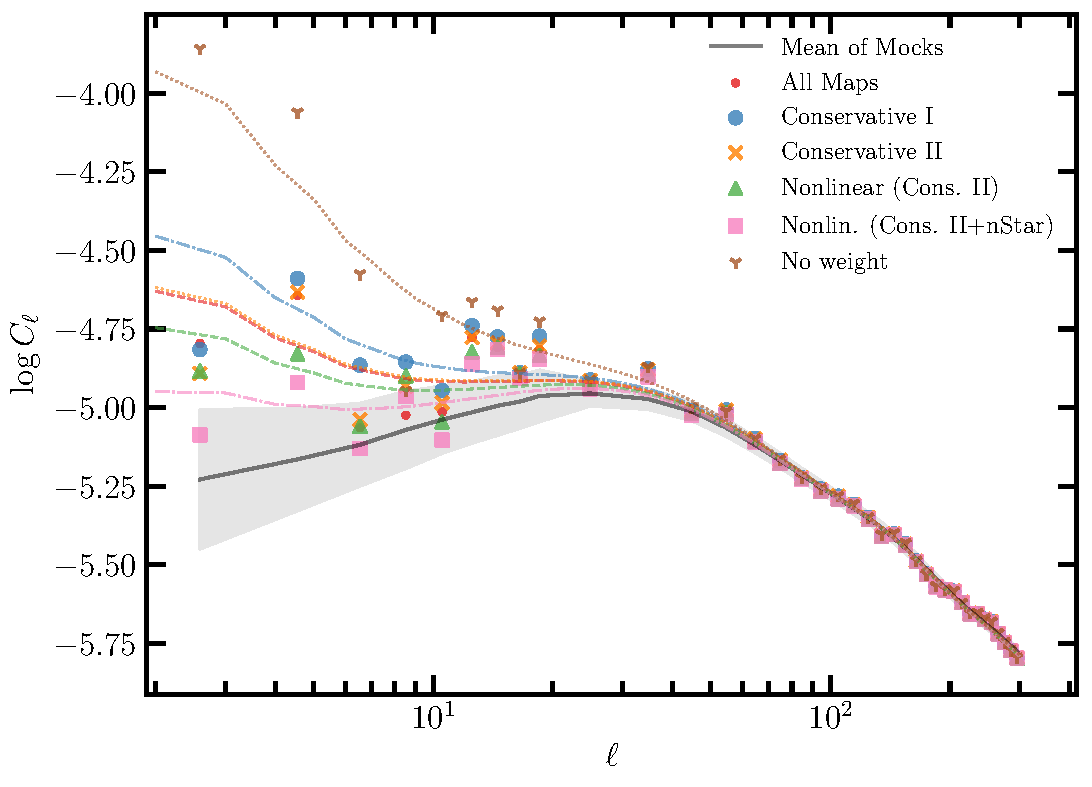
\includegraphics[width=0.47\textwidth]{figures/model_dr9.pdf} 
    \caption{The angular power spectrum of the DESI LRG targets before (\textit{No weight}) and after correcting for imaging systematics using the linear and non-linear methods. The curves represent the corresponding best-fitting theory predictions. The solid curve and grey shade respectively represent the mean power spectrum and $68\%$ error from the $\fnl=0$ mocks.}
    \label{fig:cl_dr9}
\end{figure}


\subsection{DESI imaging LRG sample}
We find that the excess clustering signal in the power spectrum of the DESI LRG targets is mitigated after correcting for the imaging systematic effects. Figure \ref{fig:cl_dr9} shows the measured power spectrum of the DESI LRG targets before and after applying imaging weights and the best-fitting theory curves. The solid line and the grey shade represent respectively the mean power spectrum and 1$\sigma$ error, estimated from the $\fnl=0$ lognormal simulations. 



The differences between various cleaning methods are significant on large scales ($\ell < 20$), but the small scale clustering measurements are consistent. By comparing \textit{linear two maps} to \textit{linear three maps}, we find that the measured clustering power on modes with $6\leq \ell < 10$ are noticeably different between the two methods. We associate the differences to the additional map for psfsize in the r-band, which is included in \textit{linear three maps}. On other scales, the differences between \textit{linear three maps} and \textit{linear eight maps} are negligible, supporting the idea that our feature selection procedure has been effective in identifying the primary maps which cause the large-scale excess clustering signal. Comparing \textit{non-linear three maps} to \textit{linear three maps}, we find that the measured spectra on $4 \leq \ell < 6$ are very different, probably indicating some non-linear spurious fluctuations with large scale characteristics due to extinction. Adding stellar density in the non-linear approach (\textit{non-linear four maps}) further reduces the excess power relative to the mock power spectrum, in particular on modes between $2\leq \ell < 4$. However, when calibrated on the lognormal simulations, we find that the over-subtraction due to stellar density is reversed after accounting for over-correction.


\subsubsection{Calibrated constraints}
All $\fnl$ constraints presented here are calibrated for the effect of over-correction using the lognormal simulations. Table \ref{tab:dr9methodcalib} describes the best-fitting and marginalized mean estimates of $\fnl$ from fitting the power spectrum of the DESI LRG targets before and after cleaning with the non-linear approach given various combinations for the imaging systematic maps. Figure \ref{fig:mcmc_dr9} shows the marginalized probability distribution for $\fnl$ in the top panel, and the $68\%$ and $95\%$ probability contours for the linear bias parameter and $\fnl$ in the bottom panel, from our sample before and after applying various corrections for imaging systematics. Overall, we find the maximum likelihood estimates to be consistent among the various cleaning methods. We obtain \mr{$33 (21) < \fnl < 61(76)$} at $68\%(95\%)$ confidence with \mr{$\chi^{2}=33.9$} for \textit{non-linear three maps} with $34$ degrees of freedom. Accounted for over-correction, we obtain \mr{$33(19) < \fnl < 62(78)$ with $\chi^{2}=34.4$ using the \textit{non-linear four maps} method which includes the additional stellar density map}. With or without stellar density, the confidence intervals are consistent with each other and significantly off from zero PNG; specifically, the probability that $\fnl$ is greater than zero, $P(\fnl >0)=99.9$ per cent. We also apply a more aggressive systematics treatment that includes regression using the nonlinear approach against the full set of imaging maps we identified, nonlinear nine maps, and find that our maximum
likelihood value changes \mout{only slightly} to \mr{$\fnl \sim 34$}, \mout{but} \mr{and} the uncertainty on $\fnl$ increases \mr{by more than a factor of two} due
to the aggressive treatment removing large-scale clustering information. For comparison, we obtain \mr{$102(86) < \fnl < 140(161)$} at $68\% (95\%)$ confidence with \mr{$\chi^{2}=45.1$} for the \textit{no weight} case.


\begin{table*}
    \caption{\mr{WIHTOUT MAG BIAS} The calibrated best-fitting, marginalized mean, and marginalized $68\%$ ($95\%$) confidence estimates for $\fnl$ from fitting the power spectrum of the DESI LRG targets before and after correcting for imaging systematic effects. The lowest mode is $\ell_{\rm min}=2$.}
   \centerline{%     
    \begin{tabular}{llllllll}
    \hline
    \hline
   &  & 	  & & $\fnl$ &  &  \\
   \cmidrule(r{.7cm}){3-6}
Footprint      & Method & 	Best fit  & Mean & $ 68\%$ CL & $ 95\%$ CL & $\chi^{2}$/dof \\
    \hline
DESI & No Weight   & $113$& $115$& $ 98<\fnl<133$& $ 84<\fnl<152$ &   44.4/34\\
DESI & Nonlinear Three Maps& $ 47$& $ 49$& $ 36<\fnl< 61$& $ 25<\fnl< 76$ &   34.6/34\\
DESI & Nonlinear Four Maps& $ 49$& $ 50$& $ 37<\fnl< 63$& $ 25<\fnl< 78$ &   35.2/34\\
DESI & Nonlinear Nine Maps& $ 50$& $ 42$& $ 13<\fnl< 69$& $-16<\fnl< 92$ &   39.5/34\\
   \hline
    \end{tabular}
}
\end{table*}


\begin{table*}
    \caption{The calibrated best-fitting, marginalized mean, and marginalized $68\%$ ($95\%$) confidence estimates for $\fnl$ from fitting the power spectrum of the DESI LRG targets before and after correcting for imaging systematic effects. The lowest mode is $\ell_{\rm min}=2$.}
    \label{tab:dr9methodcalib}
   \centerline{%     
    \begin{tabular}{llllllll}
    \hline
    \hline
   &  & 	  & & $\fnl$ &  &  \\
   \cmidrule(r{.7cm}){3-6}
Footprint      & Method & 	Best fit  & Mean & $ 68\%$ CL & $ 95\%$ CL & $\chi^{2}$/dof \\
    \hline
DESI                      & No Weight   & $   118$& $   121$& $   102<\fnl<   140$& $    86<\fnl<   161$ &   45.1/34\\
DESI                      & Nonlinear Three Maps& $    46$& $    47$& $    33<\fnl<    61$& $    21<\fnl<    76$ &   33.9/34\\
DESI                      & Nonlinear Four Maps& $    46$& $    47$& $    33<\fnl<    62$& $    19<\fnl<    78$ &   34.4/34\\
DESI                      & Nonlinear Nine Maps& $    34$& $    24$& $   -10<\fnl<    58$& $   -39<\fnl<    84$ &   39.1/34\\
   \hline
    \end{tabular}
}
\end{table*}



\begin{figure}
    \raggedleft
    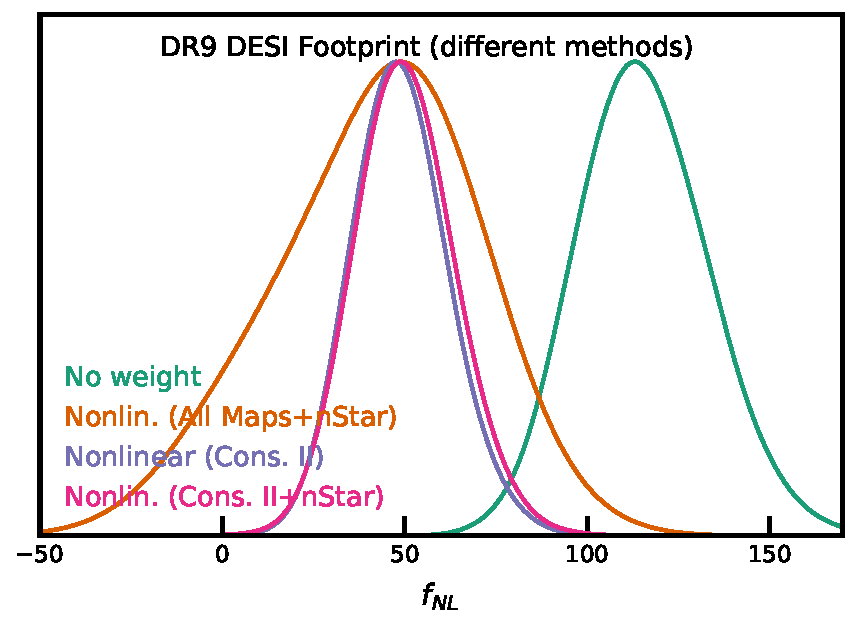
\includegraphics[width=0.439\textwidth, trim={0 1.4cm 0 0},clip]{mcmc_dr9methods1d.pdf}
    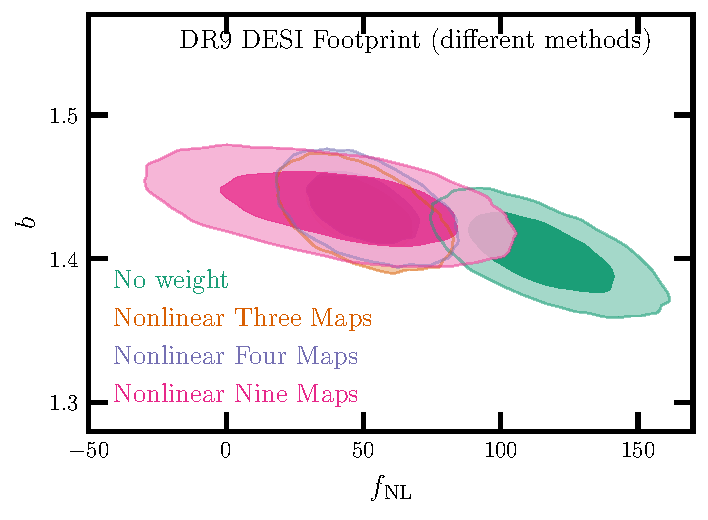
\includegraphics[width=0.47\textwidth, trim={0 0 0.15cm 0.2cm},clip]{figures/mcmc_dr9methods.pdf} 
    \caption{The calibrated constrains from the DESI LRG targets. \textit{Top}: probability distribution for $\fnl$ marginalized over the shotnoise and bias. \textit{Bottom}: $68\%$ and $95\%$ probability distribution contours for the bias and $\fnl$ from the DESI LRG targets before and after applying non-linear cleaning methods. The lognormal mocks are used to calibrate these distributions for over-correction.}\label{fig:mcmc_dr9}
\end{figure}

\subsubsection{Uncalibrated constraints: robustness tests}
Figure \ref{fig:mcmcdr9noshift} shows the probability distributions of $\fnl$ for various treatments before accounting for the over-correction effect. The method with the largest flexibility and more number of imaging systematic maps is more likely to regress out the clustering signal aggressively and return biased $\fnl$ constraints. \mout{As expected, non-linear nine maps yields the smallest maximum likelihood estimate of \mr{$\fnl=-13$}}. Our non-linear three maps returns a best-fitting estimate of \mr{$\fnl=27$} with the $68\%(95\%)$ confidence of \mr{$17(6)<\fnl <40(53)$} and \mr{$\chi^{2}=33.9$}. With the stellar density map included, non-linear four maps yields a smaller best-fitting estimates of \mr{$\fnl=14$} with the error of \mr{$5(-6)<\fnl<26(38)$}. The non-linear nine maps gives an \mr{asymmetric} posterior with the marginalized mean \mr{$\fnl=-17$}, \mr{the smallest best-fitting} estimate \mr{of $\fnl=-13$} with the error of \mr{$-31(-44)<\fnl<-3(9)$}. \mr{The differences observed in the best fitting estimates can be associated to over-correction, similar to the effect observed in the mocks (see Figure \ref{fig:contmcmc}). Therefore, the uncalibrated values should be considered with caution. For the non-linear three maps approach, without accounting for over-correction, the probability that $\fnl$ is greater than zero, $P(\fnl >0)=99.4$ per cent.}

Now we proceed to perform some robustness tests and assess how sensitive the $\fnl$ constraints are to the assumptions made in the analysis or the quality cuts applied to the data. For each case, we re-train the cleaning methods and derive new sets of imaging weights. Accordingly, for the cases where a new survey mask is applied to the data, we re-calculate the covariance matrices using the new survey mask to account for the changes in the survey window and integral constraint effects. Calibrating the mitigation biases for all of these experiments is beyond the scope of this work and redundant, as we are only interested in the relative shift in the $\fnl$ constraints after changing the assumptions. Therefore, the absolute scaling of the $\fnl$ constraints presented here are biased because of the over-correction effect. Table \ref{tab:dr9method} summarizes the uncalibrated $\fnl$ constraints from the DESI LRG targets. Our tests are as follows:

\begin{itemize}[itemindent=*]

\item \textbf{Linear methods}: Even though the linear three maps approach shows significant remaining systematics (Figure \ref{fig:chi2test} and Table \ref{tab:chi2test}), we obtain identical constraints from \textit{linear eight maps} and \textit{linear three maps}, respectively, \mr{$24(14)<\fnl<49(63)$ and $25(14)<\fnl<50(64)$} at $68\%(95\%)$ confidence. 

\item \textbf{Imaging regions}: We compare how our constraints from fitting the power spectrum of the whole DESI footprint compares to that from the power spectrum of each imaging region individually, namely BASS+MzLS, DECaLS North, and DECaLS South. Figure~\ref{fig:mcmc_dr9reg} shows the $68\%$ and $95\%$ probability contours on $\fnl$ and $b$ from each individual region, compared with that from DESI. The cleaning method here is \textit{non-linear three maps}, and the covariance matrices are estimated from the $\fnl=0$ mocks. The bias in DECaLS North is lower than the ones from DECaLS South and BASS+MzLS, which might indicate some remaining systematic effects that could not be mitigated with the available imaging systematic maps. This is because given the negative correlation between $b$ and $\fnl$, a larger value of $\fnl$ due to excess clustering power needs to be compensated by a smaller value of $b$. Overall, we find that the constraints from analyzing each imaging survey separately are consistent with each other and DESI within $68\%$ confidence. \mout{Ignoring the over-correction effect, we find that the results from the DECaLS North region to be the only one that finds PNG nonzero at greater than 95\%, which motivates follow-up studies with the spectroscopic sample of LRGs in DECaLS North.}

\item \textbf{Stellar density template (\textit{nStar})}: When not accounting for over-correction, adding the stellar density map appears to result in significant changes in the $\fnl$ constraints, e.g., compare non-linear three maps with non-linear four maps in Table \ref{tab:dr9method}. But these changes disappear when we account for the mitigation bias and we find \mout{all}\mr{both} methods recover the same maximum likelihood estimate for \mr{$\fnl \sim 46$} within $69\%$ confidence, see Table \ref{tab:dr9methodcalib}, which implies that these changes can be associated with the over-correction issue from the chance correlations between the stellar density map and large-scale structure.

\item \textbf{Pixel completeness (\textit{comp. cut})}: We discard pixels with fractional completeness less than half to assess the effect of partially complete pixels on $\fnl$. This pixel completeness cut removes $0.6\%$ of the survey area, and no changes in the $\fnl$ constraints are observed.

\item \textbf{Imaging quality (\textit{imag. cut})}: Pixels with poor photometry are removed from our sample by applying the following cuts on imaging; $E[B-V]<0.1$, $nStar < 3000$, ${\rm depth}_{g} > 23.2$, ${\rm depth}_{r} > 22.6$, ${\rm depth}_{z} > 22.5$, ${\rm psfsize}_{g}<2.5$, ${\rm psfsize}_{r}<2.5$, and ${\rm psfsize}_{z}<2$. Although these cuts remove $8\%$ of the survey mask, there is a negligible impact on the best-fitting $\fnl$ from fitting the DESI power spectrum. However, when each region \mr{power spectrum} is fit individually, the BASS+MzLS constraint shift toward higher values of $\fnl$ by approximately $\Delta \fnl \sim 10$, \mr{the DECaLS South posterior becomes highly asymmetric,} whereas \mout{the constraints from} \mr{the DECaLS North posterior} \mout{and DECaLS South} do\mr{es} not change significantly. 

\item \textbf{Covariance matrix (\textit{cov})}: We fit the power spectrum of our sample cleaned with \textit{non-linear three maps} correction, but use the covariance matrix constructed from the $\fnl=76.9$ mocks. With the alternative covariance, a \mr{$13\%$} increase in the $\sigma(\fnl)$ is observed. We also find that the best-fitting and marginalized mean estimates of $\fnl$ increase by \mr{$\Delta \fnl = 3$}. Overall, we find that the differences are not significant in comparison to the statistical precision.

\item \textbf{External maps (\textit{CALIBZ+HI})}: The neural network five maps correction includes the additional maps for HI and CALIBZ. With this correction, the best-fitting $\fnl$ increases from \mr{$41$ to $56$} for DECaLS North and from \mr{$30$ to $33$} for DECaLS South, which might suggest that adding HI and CALIBZ increases the input noise, and thus negatively impacts the performance of the neural network model. This test is not performed on BASS+MzLS due to a lack of coverage from the CALIBZ map. 

\item \textbf{Declination mask (\textit{no DEC cut})}: The fiducial mask removes the disconnected islands in DECaLS North and regions with DEC $<-30$ in DECaLS South, where there is a high likelihood of calibration issues as different standard stars are used for photometric calibrations. We analyze our sample without these cuts, and find that the best-fitting and marginalized $\fnl$ mean estimates from DECaLS South shift significantly to higher values of $\fnl$ by \mr{$\Delta \fnl \sim 15$}, which supports the case that there are remaining photometric systematics in the DECaLS South region below DEC $=-30$. On the other hand, the constraints from DECaLS North do not change significantly, indicating the islands do not induce significant contaminations.

\item \textbf{Scale dependence (\textit{varying $\ell_{\rm min}$})}: We raise the value of the lowest harmonic mode $\ell_{\rm min}$ used for the likelihood evaluation during MCMC. This is equivalent to utilizing smaller spatial scales in the measurements of the power spectrum. By doing so, we anticipate a reduction in the impact of imaging systematics on $\fnl$ inference as lower $\ell$ modes are more likely to be contaminated. Figure \ref{fig:mcmc_dr9elmin} illustrates the power spectra before and after the correction with \textit{non-linear three maps} in the top panel. The bottom panel shows the marginalized mean and $68\%$ error on $\fnl$ with \textit{non-linear three maps} for the DESI, BASS+MzLS, DECaLS North, and DECaLS South regions. We discover that a slight upward shift in the mean estimates of $\fnl$ on scales ranging from $12$ to $18$ for DECaLS North and BASS+MzLS when we utilized a higher $\ell_{\rm min}$. This outcome might imply that the imaging systematic maps do not contain enough information to help the cleaning method null out the contaminating signal in the NGC. We also find that the bump is resilient against an alternative correction, in which we apply the neural networks trained on the DECaLS South to the DECaLS North region (see \ref{ssec:ndecalsbump}). Overall, this result is contrary to what one might predict if a significant systematic-induced spike existed at the very low $\ell$\mr{, or if we had an extremely large-scale systematic leakage from the $\ell=1$ mode}. As a result, it suggests that the underlying issue is more subtle than originally anticipated.

\mr{\item \textbf{Theoretical systematics}: Our analysis is simplified by fixing the values of $p$ and $s$ to their pre-determined and estimated values. We also explore the robustness of the $\fnl$ posterior against various values of $p$, ranging between $0.55$ and $1.6$, and $s$ from $0.75$ to $1.25$. Overall, as illustrated in Figure \ref{fig:fnl_magbias}, we find that the $\fnl$ posterior to be insensitive to the value of $s$, and the impact of $p$ on $P(\fnl > 0)$ to be insignificant (see Table \ref{tab:dr9ps}).}
\end{itemize}



\begin{table*}
    \caption{\mr{WITHOUT MAG BIAS} The uncalibrated best-fitting and marginalized mean estimates for $\fnl$ from fitting the power spectrum of the DESI LRG targets before and after correcting for systematics. The estimates are not calibrated for over-correction, and thus are subject to mitigation systematics. The number of degrees of freedom is 34 (37 data points - 3 parameters). The lowest mode is $\ell=2$ and the covariance matrix is from the $\fnl=0$ clean mocks (no mitigation) except for the case with '+cov' in which the covariance matrix is from the $\fnl=76.9$ clean mocks (no mitigation).}
   \centerline{%     
    \begin{tabular}{llllllll}
    \hline
    \hline
   &  & 	  & & $\fnl$ + Mitigation Systematics &  &  \\
   \cmidrule(r{.7cm}){3-6}
Footprint                               & Method & 	Best fit  & Mean & $ 68\%$ CL & $ 95\%$ CL & $\chi^{2}$ \\
    \hline
\bf{DESI}                      & \bf{No Weight }  & $\bf{113}$& $\bf{115}$& $ \bf{98<\fnl<133}$& $ \bf{84<\fnl<152}$ &   \bf{44.4}\\
DESI                      & Linear Eight Maps& $ 36$& $ 38$& $ 26<\fnl< 49$& $ 16<\fnl< 62$ &   41.1\\
DESI                      & Linear Two Maps& $ 50$& $ 51$& $ 38<\fnl< 64$& $ 27<\fnl< 79$ &   38.8\\
\textbf{DESI}                      & \bf{Linear Three Maps}& $ \bf{37}$& $ \bf{38}$& $ \bf{26<\fnl< 50}$& $ \bf{16<\fnl< 63}$ &   \bf{39.6}\\
\textbf{DESI}                      & \textbf{Nonlinear Three Maps}& $ \bf{29}$& $ \bf{30}$& $ \bf{19<\fnl< 41}$& $  \bf{9<\fnl< 53}$ &   \bf{34.6}\\
DESI (imag. cut)          & Nonlinear Three Maps& $ 29$& $ 31$& $ 19<\fnl< 42$& $  9<\fnl< 55$ &   35.8\\
DESI (comp. cut)          & Nonlinear Three Maps& $ 28$& $ 29$& $ 18<\fnl< 40$& $  9<\fnl< 53$ &   34.5\\
DESI                      & Nonlinear Four Maps& $ 17$& $ 18$& $  8<\fnl< 27$& $ -2<\fnl< 38$ &   35.2\\
DESI                      & Nonlinear Nine Maps& $ -6$& $ -9$& $-21<\fnl<  2$& $-34<\fnl< 12$ &   39.5\\
DESI                     & Nonlinear Three Maps+$f_{\rm NL}=76.9$ Cov& $ 32$& $ 33$& $ 21<\fnl< 45$& $ 11<\fnl< 59$ &   33.5\\
\hline
\bf{BASS+MzLS}                 & \bf{Nonlinear Three Maps}& $ \bf{15}$& $ \bf{19}$& $ \bf{-1<\fnl< 39}$& $\bf{-19<\fnl< 64}$ & \bf{35.6}\\
BASS+MzLS                 & Nonlinear Four Maps& $ 13$& $ 15$& $ -5<\fnl< 36$& $-25<\fnl< 59$ &   34.7\\
BASS+MzLS                 & Nonlinear Nine Maps& $ -4$& $ -6$& $-27<\fnl< 14$& $-47<\fnl< 34$ &   36.8\\
BASS+MzLS (imag. cut)     & Nonlinear Three Maps& $ 25$& $ 29$& $  6<\fnl< 52$& $-14<\fnl< 81$ &   36.2\\
BASS+MzLS (comp. cut)     & Nonlinear Three Maps& $ 17$& $ 21$& $  0<\fnl< 42$& $-18<\fnl< 67$ &   35.8\\
\bf{DECaLS North}              & \bf{Nonlinear Three Maps}& $ \bf{41}$& $ \bf{45}$& $ \bf{23<\fnl< 67}$& $  \bf{5<\fnl< 93}$ & \bf{41.1}\\
DECaLS North              & Nonlinear Four Maps& $ 31$& $ 35$& $ 14<\fnl< 56$& $ -6<\fnl< 81$ &   41.2\\
DECaLS North              & Nonlinear Five Maps& $ 55$& $ 60$& $ 37<\fnl< 84$& $ 18<\fnl<113$ &   38.4\\
DECaLS North              & Nonlinear Nine Maps& $  1$& $ -6$& $-30<\fnl< 17$& $-53<\fnl< 36$ &   45.1\\
DECaLS North (no DEC cut) & Nonlinear Three Maps& $ 41$& $ 45$& $ 24<\fnl< 66$& $  6<\fnl< 91$ &   40.7\\
DECaLS North (imag. cut)  & Nonlinear Three Maps& $ 43$& $ 48$& $ 25<\fnl< 72$& $  5<\fnl<101$ &   35.1\\
DECaLS North (comp. cut)  & Nonlinear Three Maps& $ 41$& $ 45$& $ 22<\fnl< 67$& $  4<\fnl< 94$ &   41.4\\
\bf{DECaLS South}              & \bf{Nonlinear Three Maps}& $ \bf{31}$& $ \bf{33}$& $ \bf{15<\fnl< 52}$& $ \bf{-5<\fnl< 74}$ &   \bf{30.2}\\
DECaLS South              & Nonlinear Four Maps& $ 14$& $  6$& $-21<\fnl< 30$& $-54<\fnl< 50$ &   31.9\\
DECaLS South              & Nonlinear Five Maps& $ 34$& $ 37$& $ 18<\fnl< 57$& $ 0<\fnl< 81$ &   30.8\\
DECaLS South              & Nonlinear Nine Maps& $-37$& $-32$& $-49<\fnl<-14$& $-65<\fnl<  8$ &   31.5\\
DECaLS South (no DEC cut) & Nonlinear Three Maps& $ 44$& $ 47$& $ 30<\fnl< 63$& $ 16<\fnl< 83$ &   23.8\\
DECaLS South (imag. cut)  & Nonlinear Three Maps& $ 26$& $ 23$& $  3<\fnl< 48$& $-58<\fnl< 71$ &   30.0\\
DECaLS South (comp. cut)  & Nonlinear Three Maps& $ 30$& $ 32$& $ 13<\fnl< 52$& $ -9.78<\fnl< 74$ &   29.7\\
   \hline
    \end{tabular}}
\end{table*}



\begin{table*}
    \caption{The uncalibrated best-fitting and marginalized mean estimates for $\fnl$ from fitting the power spectrum of the DESI LRG targets before and after correcting for systematics. The estimates are not calibrated for over-correction, and thus are subject to mitigation systematics. The number of degrees of freedom is 34 (37 data points - 3 parameters). The lowest mode is $\ell=2$ and the covariance matrix is from the $\fnl=0$ clean mocks (no mitigation) except for the case with '+ Cov' in which the covariance matrix is from the $\fnl=76.9$ clean mocks (no mitigation).}
    \label{tab:dr9method}
   \centerline{%     
    \begin{tabular}{llllllll}
    \hline
    \hline
   &  & 	  & & $\fnl$ + Mitigation Systematics &  &  \\
   \cmidrule(r{.7cm}){3-6}
Footprint                               & Method & 	Best fit  & Mean & $ 68\%$ CL & $ 95\%$ CL & $\chi^{2}$ \\
    \hline
\textbf{DESI}                      & \textbf{No Weight}   & $   \bf{118}$& $   \bf{121}$& $   \bf{102<\fnl<   140}$& $    \bf{86<\fnl<   161}$ &   \bf{45.1}\\
DESI                      & Linear Two Maps& $    49$& $    51$& $    37<\fnl<    65$& $    25<\fnl<    80$ &   37.9\\
\textbf{DESI}                      & \textbf{Linear Three Maps}& $    \textbf{36}$& $    \textbf{37}$& $    \bf{25<\fnl<50}$& $    \bf{14<\fnl<    64}$ &   \bf{38.6}\\
DESI                      & Linear Eight Maps& $    35$& $    37$& $    24<\fnl<    49$& $    14<\fnl<    63$ &   40.4\\
\bf{DESI}                      & \bf{Nonlinear Three Maps}& $    \bf{27}$& $    \bf{28}$& $    \bf{17<\fnl<    40}$& $     \bf{6<\fnl<    53}$ &   \bf{33.9}\\
DESI (imag. cut)          & Nonlinear Three Maps& $    28$& $    30$& $    17<\fnl<    42$& $     6<\fnl<    56$ &   35.4\\
DESI (comp. cut)          & Nonlinear Three Maps& $    27$& $    28$& $    16<\fnl<    40$& $     6<\fnl<    53$ &   33.9\\
DESI                      & Nonlinear Four Maps& $    14$& $    15$& $     5<\fnl<    26$& $    -6<\fnl<    38$ &   34.4\\
DESI                      & Nonlinear Nine Maps& $   -13$& $   -17$& $   -31<\fnl<    -3$& $   -44<\fnl<     9$ &   39.1\\
DESI                     & Nonlinear Three Maps+$f_{\rm NL}=76.92$ Cov& $    30$& $    31$& $    18<\fnl<    44$& $     7<\fnl<    59$ &   32.8\\
\hline
\bf{BASS+MzLS}                 & \bf{Nonlinear Three Maps}& $    \bf{13}$& $    \bf{16}$& $    \bf{-6<\fnl<    38}$& $   \bf{-28<\fnl<64}$ &   \bf{34.9}\\
BASS+MzLS                 & Nonlinear Four Maps& $    10$& $    12$& $   -11<\fnl<    34$& $   -35<\fnl<    59$ &   34.1\\
BASS+MzLS                 & Nonlinear Nine Maps& $    -9$& $   -13$& $   -37<\fnl<    10$& $   -59<\fnl<    32$ &   36.4\\
BASS+MzLS (imag. cut)     & Nonlinear Three Maps& $    23$& $    26$& $     1<\fnl<    51$& $   -23<\fnl<    81$ &   35.8\\
BASS+MzLS (comp. cut)     & Nonlinear Three Maps& $    14$& $    18$& $    -5<\fnl<    41$& $   -27<\fnl<    68$ &   35.2\\
\hline
\bf{DECaLS North}              & \bf{Nonlinear Three Maps}& $    \bf{41}$& $    \bf{45}$& $    \bf{21<\fnl<    69}$& $    \bf{-1<\fnl<    98}$ &   \bf{40.8}\\
DECaLS North              & Nonlinear Four Maps& $    30$& $    32$& $    10<\fnl<    56$& $   -18<\fnl<    83$ &   40.9\\
DECaLS North              & Nonlinear Five Maps& $    56$& $    62$& $    36<\fnl<    88$& $    15<\fnl<   121$ &   38.3\\
DECaLS North              & Nonlinear Nine Maps& $    -4$& $   -13$& $   -40<\fnl<    13$& $   -64<\fnl<    36$ &   44.6\\
DECaLS North (no DEC cut) & Nonlinear Three Maps& $    41$& $    45$& $    22<\fnl<    68$& $     1<\fnl<    96$ &   40.4\\
DECaLS North (imag. cut)  & Nonlinear Three Maps& $    43$& $    48$& $    22<\fnl<    75$& $    -1<\fnl<   107$ &   34.9\\
DECaLS North (comp. cut)  & Nonlinear Three Maps& $    40$& $    44$& $    20<\fnl<    68$& $    -2<\fnl<    97$ &   41.2\\
\hline
\bf{DECaLS South}              & \bf{Nonlinear Three Maps}& $    \bf{30}$& $    \bf{31}$& $    \bf{11<\fnl<    53}$& $   \bf{-28<\fnl<    76}$ &   \bf{30.2}\\
DECaLS South              & Nonlinear Four Maps& $   -42$& $    -5$& $   -44<\fnl<    27$& $   -70<\fnl<    49$ &   33.4\\
DECaLS South              & Nonlinear Five Maps& $    33$& $    36$& $    15<\fnl<    58$& $    -7<\fnl<    84$ &   30.7\\
DECaLS South              & Nonlinear Nine Maps& $   -43$& $   -40$& $   -58<\fnl<   -21$& $   -75<\fnl<     3$ &   31.3\\
DECaLS South (no DEC cut) & Nonlinear Three Maps& $    44$& $    46$& $    29<\fnl<    64$& $    14<\fnl<    85$ &   23.7\\
DECaLS South (imag. cut)  & Nonlinear Three Maps& $    26$& $    15$& $   -19<\fnl<    47$& $   -84<\fnl<    72$ &   30.0\\
DECaLS South (comp. cut)  & Nonlinear Three Maps& $    29$& $    28$& $     8<\fnl<    52$& $   -41<\fnl<    75$ &   29.7\\
   \hline
    \end{tabular}}
\end{table*}





\begin{figure}
    \centering
    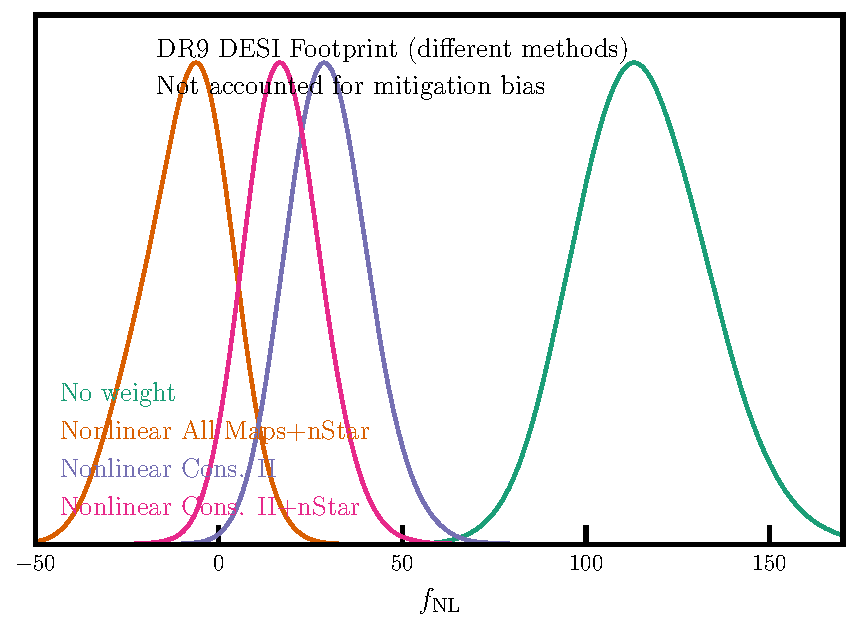
\includegraphics[width=0.45\textwidth]{figures/mcmc_dr9methods1dnoshift.pdf}
    \caption{Same as Figure \ref{fig:mcmc_dr9} but without accouting for over-correction. }
    \label{fig:mcmcdr9noshift}
\end{figure}
\begin{figure}
    \centering
    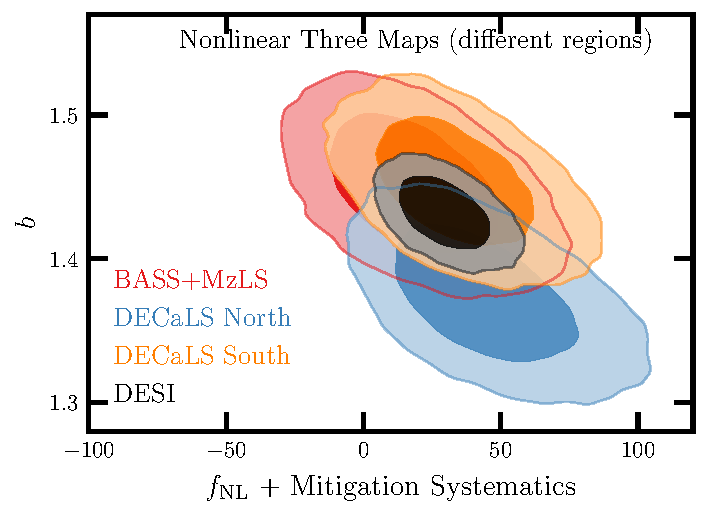
\includegraphics[width=0.45\textwidth]{figures/mcmc_dr9regions.pdf} 
    \caption{The uncalibrated 2D constraints from the DESI LRG targets for each imaging survey compared with that for the whole DESI footprint. The dark and light shades represent the $68\%$ and $95\%$ confidence intervals, respectively.}\label{fig:mcmc_dr9reg}
\end{figure}
\begin{figure*}
    \centering
    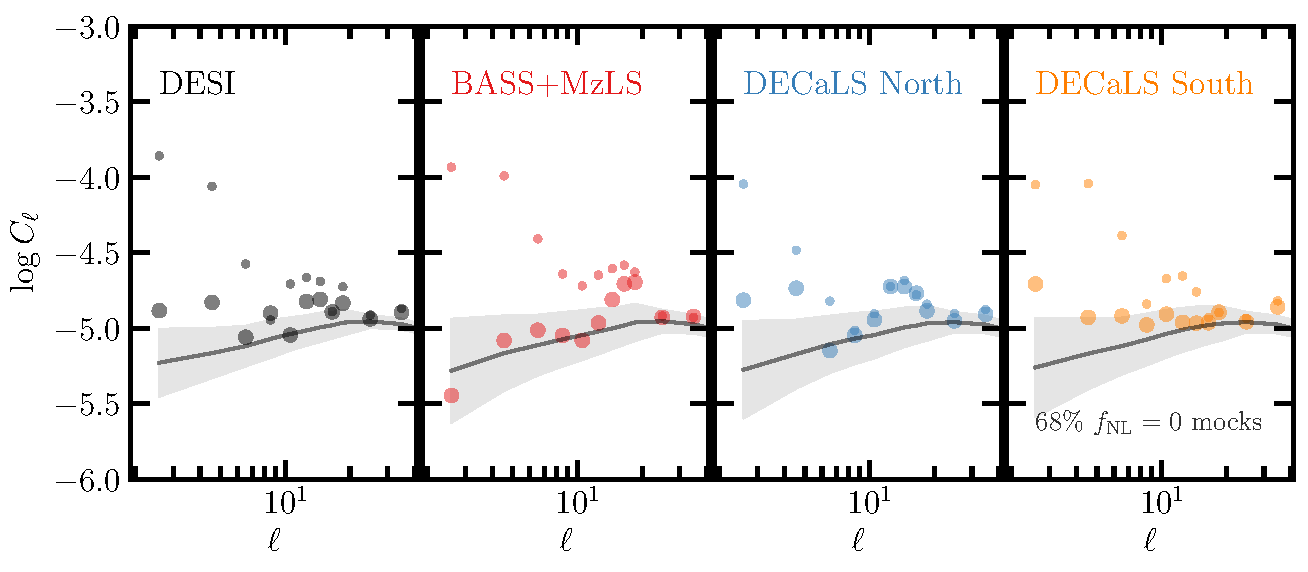
\includegraphics[width=0.9\textwidth]{figures/cldr9_lowell.pdf}
    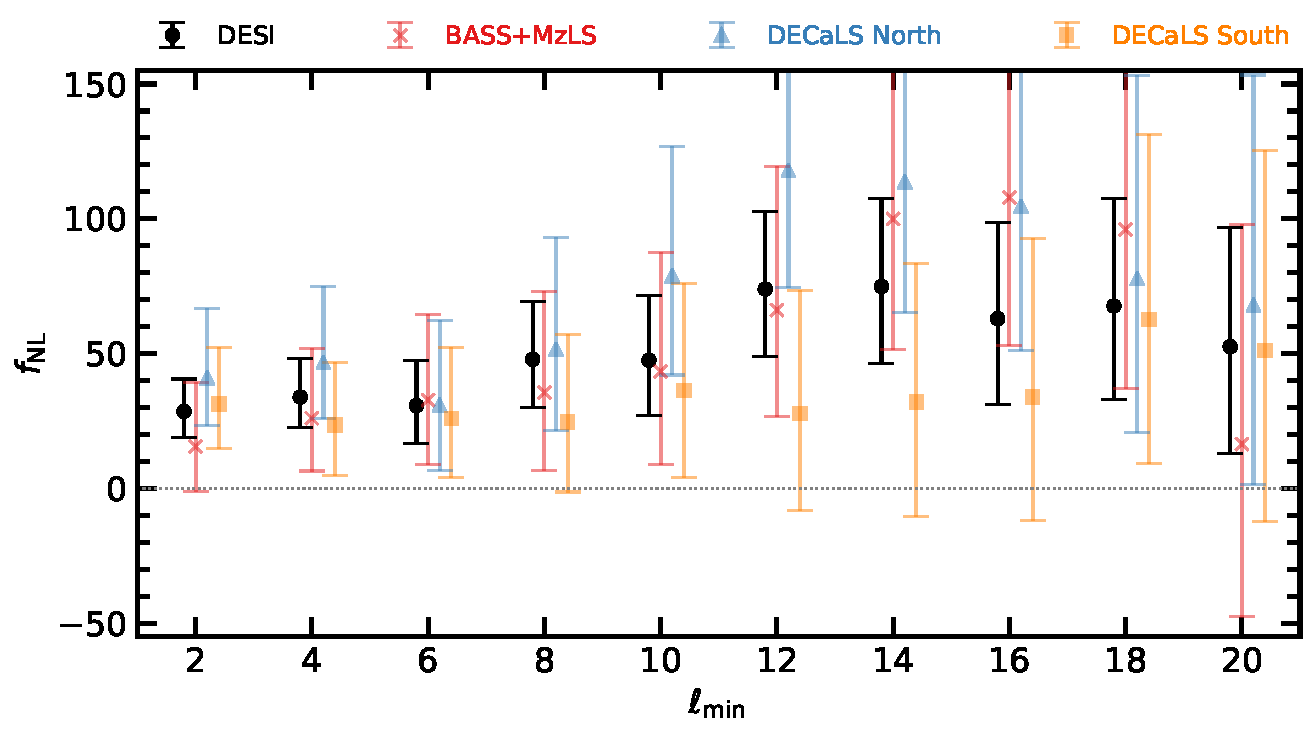
\includegraphics[width=0.9\textwidth]{figures/fnl_elmin.pdf}  
    \caption{Top: The measured power spectrum of the DESI LRG targets before (solid curves) and after \textit{non-linear three maps} (scatter points) for the DESI, BASS+MzLS, DECaLS North, and DECaLS South regions. Bottom: The uncalibrated $\fnl$ constraints vs the lowest $\ell$ mode used for fitting $\fnl$. The points represent marginalized mean estimates of $\fnl$ and error bars represent $68$\% confidence estimated from the $\fnl=0$ mocks. The scaling of $\fnl$ is not calibrated to account for over-correction caused by mitigation.}\label{fig:mcmc_dr9elmin}
\end{figure*}

\begin{figure}
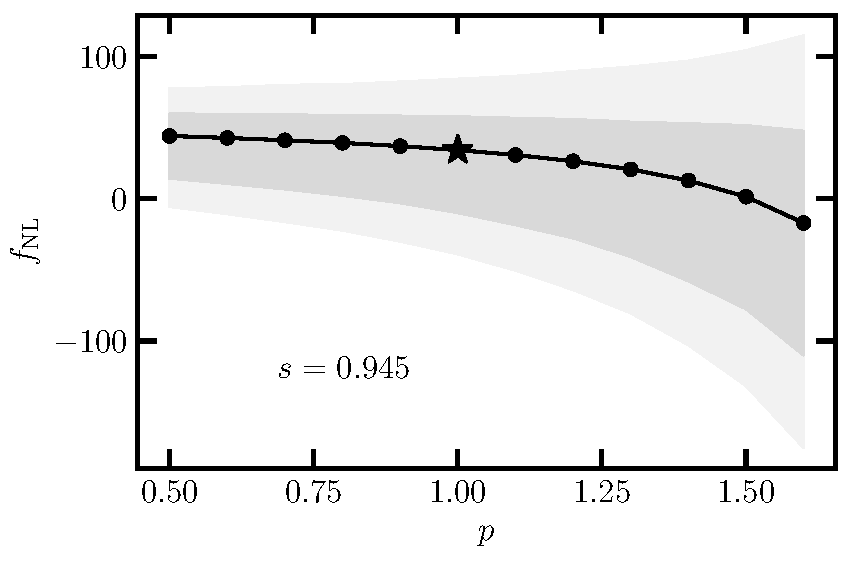
\includegraphics[width=0.45\textwidth]{figures/fnl_p.pdf}
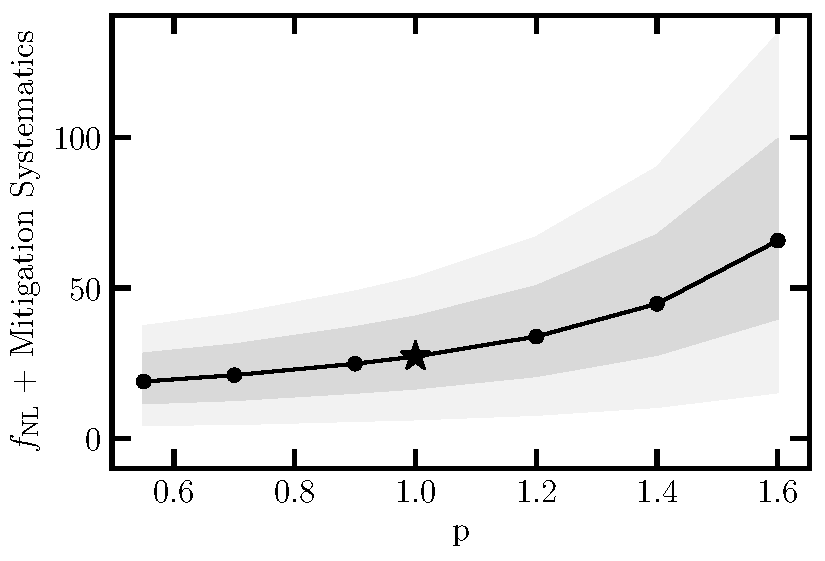
\includegraphics[width=0.45\textwidth]{figures/fnl_p2.pdf}
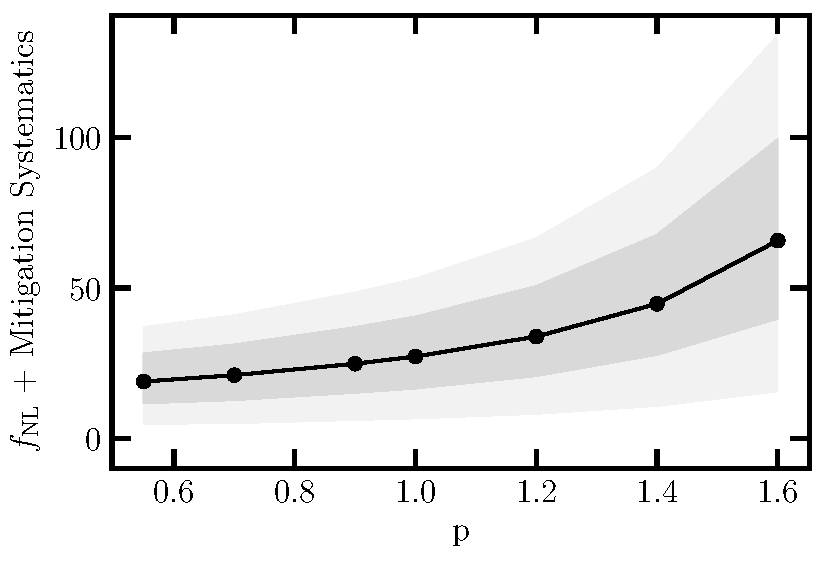
\includegraphics[width=0.45\textwidth]{figures/fnl_magbias.pdf}
\caption{\mr{Best fit estimates and $68\%$ ($95\%$) error on $\fnl$ from fitting the DESI DR9 LRG sample using the non-linear three maps cleaning approach. We find a weak dependence on $p$ but negligible impact on $s$.}}\label{fig:fnl_magbias}
\end{figure}




\begin{table*}
    \caption{The uncalibrated best-fitting and marginalized mean estimates for $\fnl$ from fitting the power spectrum of the DESI LRG targets using various values for hyper-parameters, $p$ and $s$. In each case we fix one hyper-parameter to its fiducial value ($p=1$ and $s=0.945$) while changing the other. The estimates are not calibrated for over-correction, and thus are subject to mitigation systematics. The number of degrees of freedom is 34 (37 data points - 3 parameters). The lowest mode is $\ell=2$ and the covariance matrix is from the $\fnl=0$ clean mocks (no mitigation).}
    \label{tab:dr9ps}
   \centerline{%     
    \begin{tabular}{llllllll}
    \hline
    \hline
   &  & 	  & & $\fnl$ + Mitigation Systematics &  &  \\
   \cmidrule(r{.7cm}){3-6}
Footprint                               & Method & 	Best fit  & Mean & $ 68\%$ CL & $ 95\%$ CL & $\chi^{2}$ \\
0.55                                    & $    19$& $    20$& $    12<\fnl<    28$& $     5<\fnl<    37$ &   33.9\\
0.7                                     & $    21$& $    22$& $    13<\fnl<    31$& $     5<\fnl<    41$ &   33.9\\
0.9                                     & $    25$& $    26$& $    15<\fnl<    37$& $     6<\fnl<    49$ &   33.9\\
1.0                                     & $    27$& $    28$& $    17<\fnl<    40$& $     6<\fnl<    53$ &   33.9\\
1.2                                     & $    34$& $    36$& $    21<\fnl<    50$& $     8<\fnl<    67$ &   33.9\\
1.4                                     & $    45$& $    48$& $    28<\fnl<    67$& $    11<\fnl<    90$ &   33.9\\
1.6                                     & $    66$& $    70$& $    40<\fnl<    99$& $    15<\fnl<   134$ &   33.9\\
\hline
0.75                                    & $    28$& $    30$& $    18<\fnl<    41$& $     8<\fnl<    54$ &   34.1\\
0.80                                    & $    28$& $    29$& $    17<\fnl<    41$& $     7<\fnl<    54$ &   34.1\\
0.85                                    & $    27$& $    29$& $    18<\fnl<    41$& $     8<\fnl<    54$ &   34.0\\
0.90                                    & $    27$& $    29$& $    17<\fnl<    41$& $     7<\fnl<    53$ &   34.0\\
0.945                                   & $    27$& $    28$& $    17<\fnl<    40$& $     6<\fnl<    53$ &   33.9\\
1.00                                    & $    27$& $    28$& $    17<\fnl<    40$& $     6<\fnl<    54$ &   33.9\\
1.05                                    & $    27$& $    28$& $    16<\fnl<    40$& $     6<\fnl<    54$ &   33.8\\
1.10                                    & $    27$& $    28$& $    16<\fnl<    40$& $     5<\fnl<    54$ &   33.8\\
1.15                                    & $    26$& $    28$& $    16<\fnl<    40$& $     5<\fnl<    53$ &   33.7\\
1.20                                    & $    26$& $    28$& $    15<\fnl<    40$& $     5<\fnl<    54$ &   33.7\\
1.25                                    & $    26$& $    27$& $    15<\fnl<    40$& $     4<\fnl<    53$ &   33.7\\
   \hline
    \end{tabular}}
\end{table*}